\begin{center}
    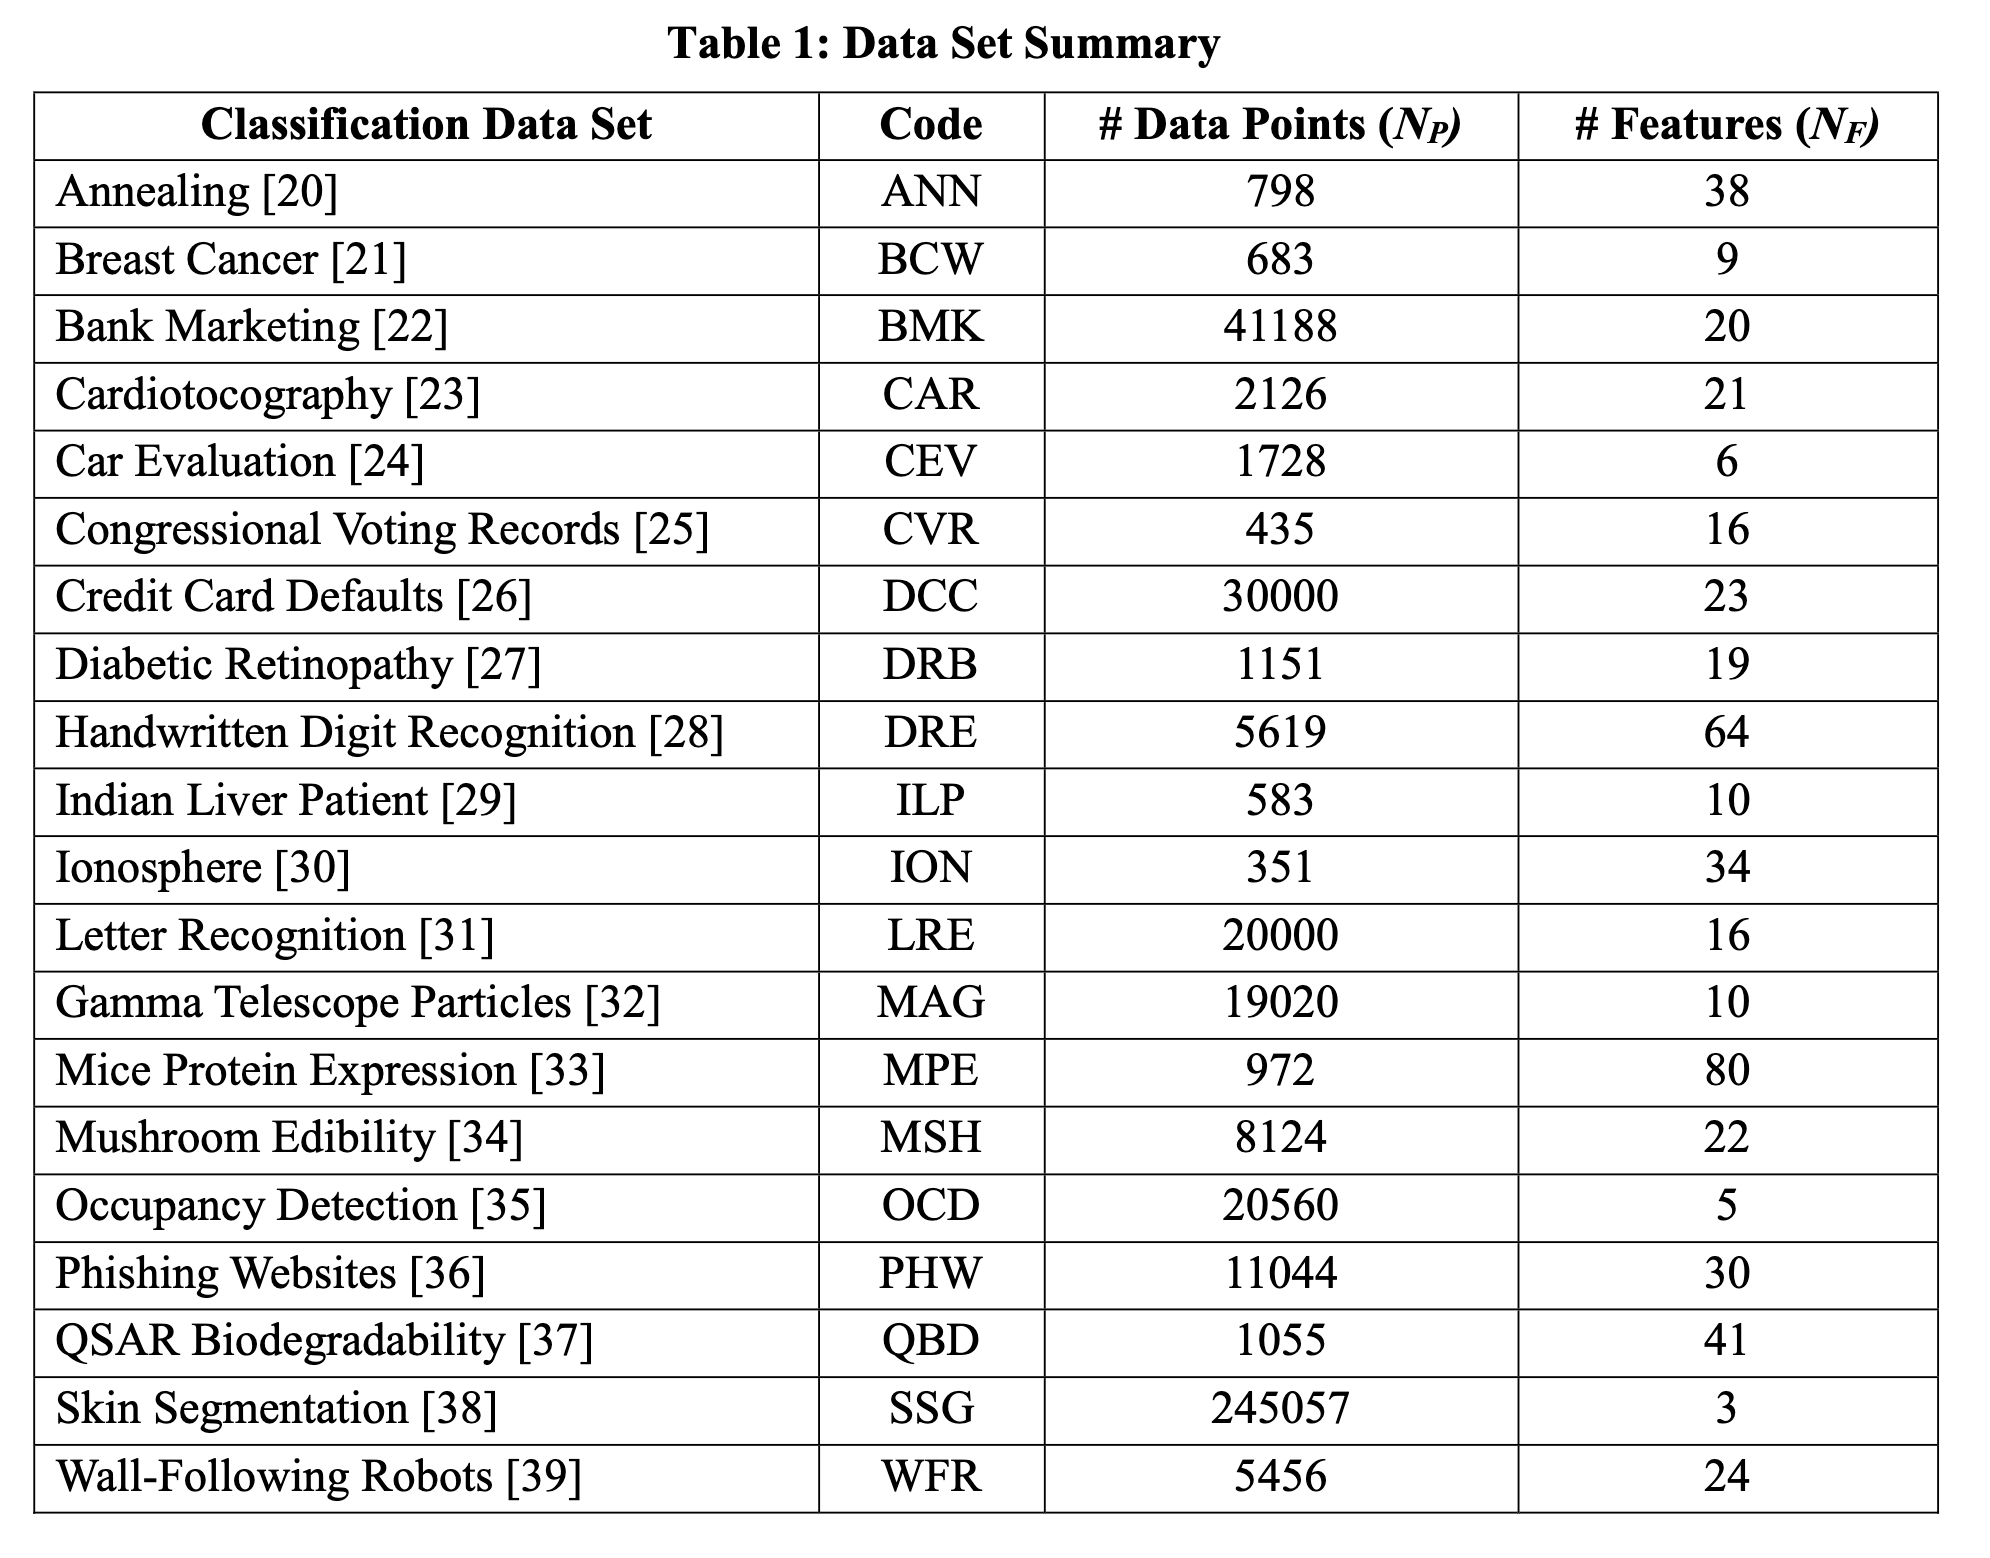
\includegraphics[width=\textwidth]{graphics/beispiel_grafik_datensaetze.png}
\end{center}
I could do something of that sort for my own data sets

\newpage
We also gathered several other characteristics of each data set, including number of categorical features (NCAT), number of continuous features (NCONT), proportion of features that are categorical (RCAT), number of target classes (NC), minimum single-class proportion (CMIN), and class imbalance (IC). The latter is a measure of the difference in actual and expected proportion of the least common target class (L) and its expected value (LE); i.e., I = (LE – L)/LE. These values are shown in Table 2.

\begin{center}
    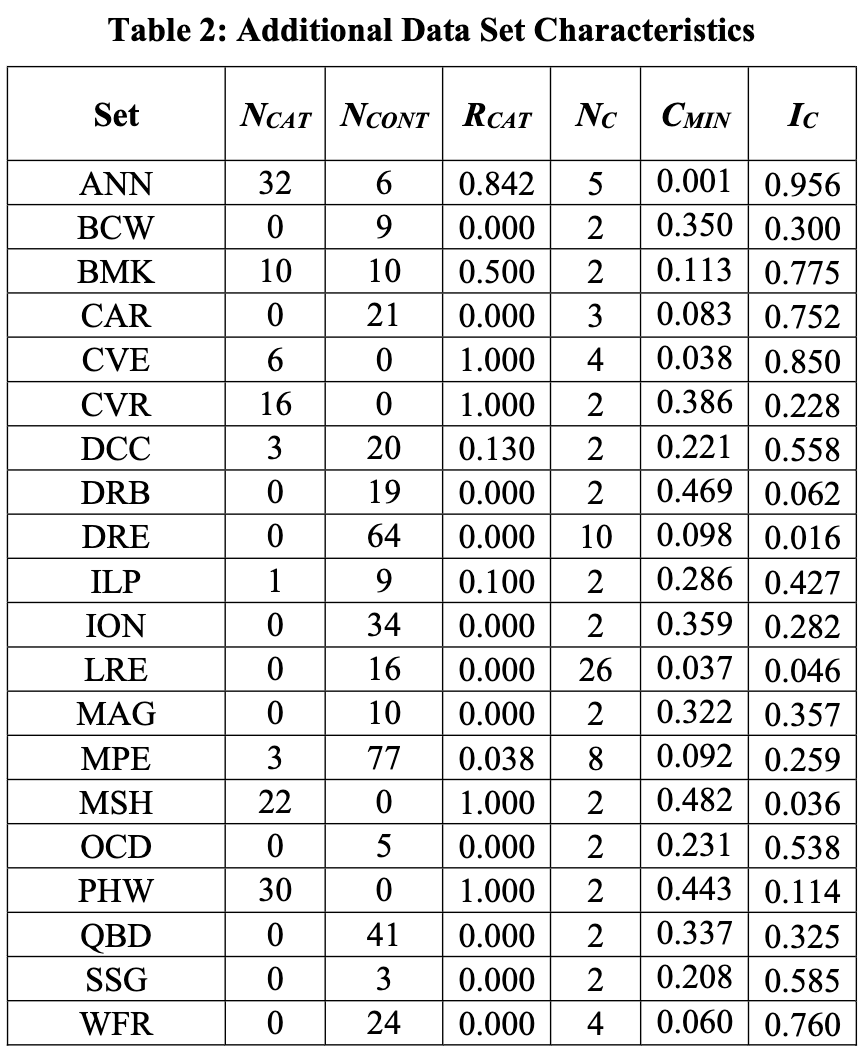
\includegraphics[width=0.5\textwidth]{graphics/variablen_analyse_datensaetze.png}
\end{center}

During the MLP training experiments, several configurations were evaluated to optimize performance. Initially, the model was trained using only the CPU, which proved too slow for practical use. Switching to CUDA-based GPU training introduced a new 
issue: the default batch size of 128 provided by \texttt{scikit-learn} resulted in training times even slower than on CPU, due to the overhead of frequent small data transfers to the GPU.

Increasing the batch size to 8,192 significantly reduced training time. Further tuning of this parameter did not yield improvements, so this value was retained. Additionally, \texttt{pin\_memory=True} was evaluated, which locks data in RAM to accelerate CPU-to-GPU transfers. However, this option also led to slower training, likely because the MLP architecture is not complex enough to benefit from the reduced transfer overhead. These experiments led to the final configuration used for all reported MLP results.

\chapter{Experimental Design}
This chapter outlines the experimental design used to evaluate the ecological efficiency of different machine learning classification algorithms. It describes the datasets, models, evaluation metrics, hyperparameter tuning and measurement setup that form the basis of this empirical analysis.

\section{Research Questions}
The main research question that this study wants to find the answer to, is: \textit{How does the trade-off between energy consumption and predictive performance vary across Random Forest, XGBoost, and MLP when model complexity and dataset size are systematically varied?}
Further the following Sub-questions will be answered in the progress of this thesis:
\begin{itemize}
    \item Under what conditions do the resource consumption of more complex models exceed the achievable accuracy gain over simpler baselines?
    \item How does energy consumption and CO2 output scale with increasing neural network complexity (number of layers and neurons)?
    \item How does energy consumption differ between CPU-based and GPU-based training for equivalent tasks?
    \item How does reducing the number of training instances on large datasets affect model accuracy and energy consumption across different algorithms?
\end{itemize}

To answer these questions multiple classification algorithms and datasets were used in the experimental phase of this empirical analysis.

\section{Datasets}


